\chapter{Einleitung}
\label{cha:einleitung}

In dieser Dokumentation wird die Entwicklung einer Quartett-App im Rahmen des Anwendungsfaches ``Mobile Application Lab'' an der Universität Ulm vorgestellt und die dabei entwickelte Anwendung präsentiert.\\

\begin{figure}[htp]
	\centering
  	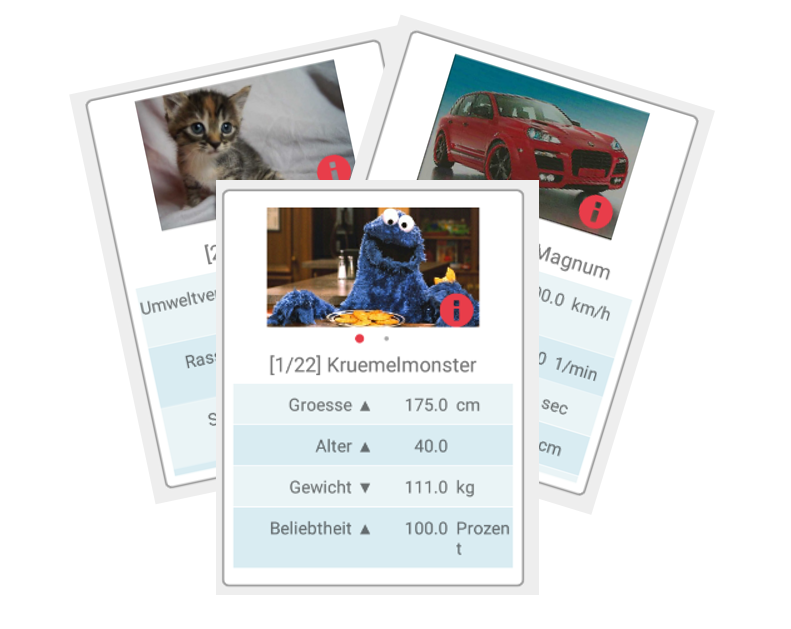
\includegraphics[width=0.4\textwidth]{img/quartett42_logo.png}
	\caption{Quartett42 Logo}
	\label{figure:quartett42logo}
\end{figure}

% Abschnitt: Problemstellung
\section{Motivation und Problemstellung}
\label{sec:einleitung:problemstellung}

Die Problemstellung wurde uns im Rahmen dieses Projektes schon gegeben, da wir uns auf die Entwicklung einer Quartett-App für Smartphones konzentrieren sollten. Das beliebte Kartenspiel soll für ein Smartphone umgesetzt werden und so zu jeder Zeit und an jedem Ort auch komplett ohne physische Karten spielbar sein.

Beim Betrachten des aktuellen Marktes für Quartett-Apps fällt schnell die Vielzahl an verschiedenen Apps auf. Diese weisen nach genauerer Untersuchung jedoch teilweise erhebliche Mängel auf. So sind manche von ihnen sehr veraltet und funktionieren nicht mehr richtig auf neueren Smartphone-Modellen. Auch entsprechen diese inhaltlich nicht unseren Vorstellungen einer guten Quartett-App. Sie sind sehr beschränkt, was die verschiedenen Spielmodi angeht, und enthalten meist nur ein einziges Kartendeck oder nur Decks aus einem bestimmten Themengebiet. In diesem Punkt wollen wir uns von den existierenden Apps absetzen.

% Abschnitt: Zielsetzung
\section{Zielsetzung}
\label{sec:einleitung:zielsetzung}

Wir wollen also die Nachfrage des Marktes ausnutzen und eine eigene Quartett-Anwendung erstellen. Diese wollen wir auf Basis von Android und Java entwickeln. Dabei geht es uns primär darum, den Umgang mit den neuen Techniken zu erlernen und Erfahrung im Programmieren von Android-Anwendungen zu erlangen, sodass wir diese nach Abschluss des Projektes beherrschen.

Inhaltlich möchten wir eine Quartett-App entwickeln, die sich im Einzelspielermodus wie ein richtiges Quartett spielen lässt. Sie soll verschiedene Spielmodi haben, welche frei konfigurierbar sein sollen. Zudem soll die App nicht auf ein Deck oder einen Themenbereich beschränkt sein. Dies soll durch einen ``Deckcreator'' und eine Funktion zum hoch- und herunterladen von Decks realisiert werden. Die Anwendung soll zudem die Möglichkeit bieten, alle Karten anzugucken sowie laufende Spiele zu unterbrechen. Dabei soll die App benutzerfreundlich sein und schön aussehen, sowie auf dem Großteil der momentan verwendeten Android-Versionen lauffähig sein.

% Abschnitt: Struktur der Arbeit
\section{Struktur der Arbeit}
\label{sec:einleitung:struktur}

In dieser Dokumentation werden zuerst die grundlegenden Quartett-Spielregeln erklärt, das Betriebssystem Android vorgestellt, sowie unsere verwendeten Frameworks präsentiert. Den Hauptteil bildet das Kapitel über die Implementierung, worin unsere App im Allgemeinen und mit ihren Besonderheiten vorstellt wird. Außerdem wird darin unsere Architektur gezeigt und auf Schwierigkeiten eingegangen, die während der Implementierungsphase auftraten. Darauf folgt ein Abgleich der Anforderungen mit der tatsächlichen Implementierung, und schließlich eine Zusammenfassung und ein Ausblick auf die Zukunft des Projektes.\\
